\documentclass[main.tex]{subfiles}

\begin{document}

\section{Power Control System}

\textit{This section will go over the \gls{pcs}, how it is constructed and describe how it functions. It will go into detail on the three parts that make up the \gls{pcs}, which is client software, \gls{fpga} and \gls{mb}. The focus will be on how the \gls{fpga} and microcontroller interfaces relates to the client software.}

The \acrfull{pcs} is the name of the modules responsible for powering the strings in the \gls{dtc}, monitor and control their temperature and power usage. The system is made of three parts, the client software on the computer, an \gls{fpga} translation layer using IPbus firmware, and a \acrlong{mb} with a microcontroller. The \gls{mb} delivers the power to the strings and also measures and monitors the strings temperature and current usage. The\gls{mb} design and microcontroller software was developed by Birger Olsen. The \gls{fpga} is a translation layer between the client software and \gls{mb}s, it uses IPbus firmware to safely and reliably transmit data packets from software to \gls{mb}. A single \gls{fpga} is used to transmit data to all 43 \gls{mb}s, meaning it must have the architecture to process data packets for every board. The \gls{fpga} design is made by Martin Eggen and Jakob Hauser. The software on the computer is the monitoring and configuration system, responsible for configuring the \gls{mb}s through the \gls{fpga} and monitor the strings, giving the user information on the performance of the strings. This control system on the software side will be discussed more in \autoref{section: monitoring} and \autoref{section: configuration}. A figure of the \gls{pcs} is shown in \autoref{fig: PCS_overview}.  \notinmain{sett bachelorgutta sitt bilde av pcs her og ta denne figuren inn i client software kapittelet istedenfor}

\begin{figure}[!htpb]
    \centering
    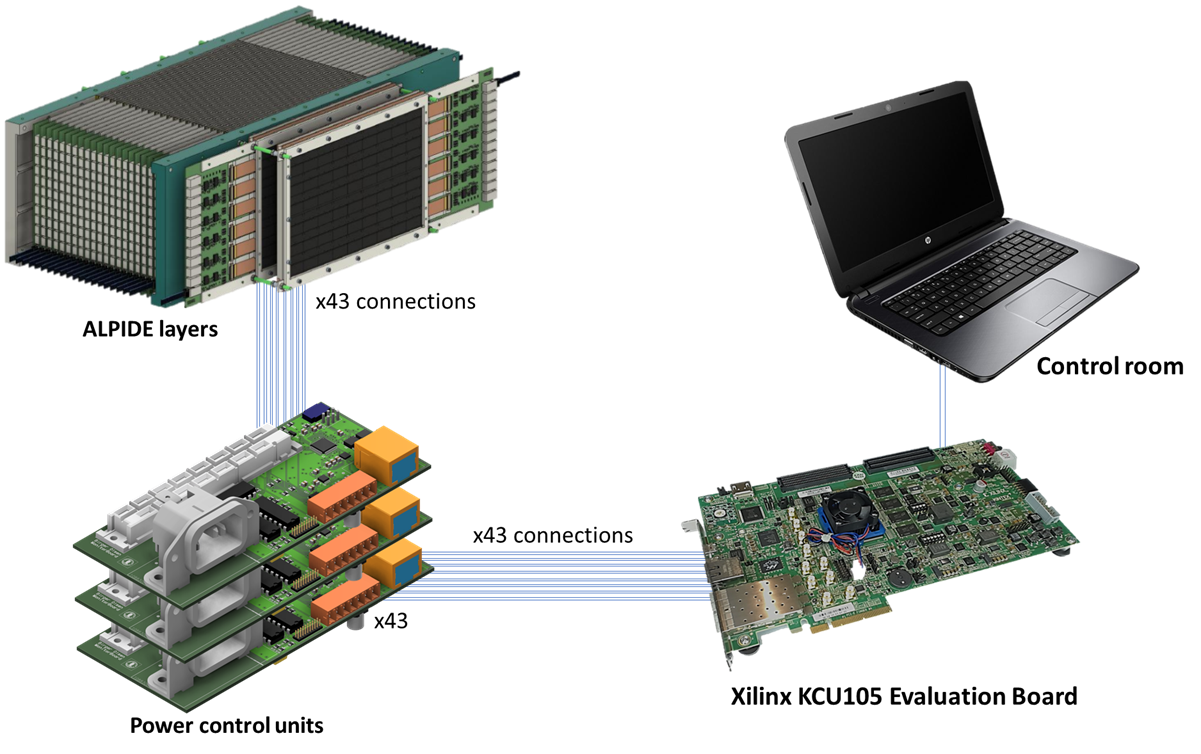
\includegraphics[width=15cm]{images/PowerDeliverySystemOverview.png}
    \caption{Overview of the PCS components.}
    \label{fig: PCS_overview}
\end{figure}
\FloatBarrier

The "Control room" is the computer with the IPbus software that can communicate with the \gls{fpga} in this instance. The "control room" will both handle the \gls{pcs} and the readout of the ALPIDE-chips. We currently have a prototype implementation of the \gls{pcs}, with software for communication, connected to the KCU105 evaluation board. The \gls{mb} is still in development, so a Curiosity Nano development kit was used to verify the connection between the KCU105 and microcontroller software. An image of this setup is shown in Figure ??.


There is obviously no connection between the microcontroller and the \gls{dtc} yet, and there is only one layer connected, but it still allows us to do performance tests that will give us good estimations of the final product.

This chapter will go over the different design approaches for each part of the \gls{pcs}, going over the requirements for the system and how it is implemented.

\subsection{Client Software}

The client software is made of a monitoring system, a configuration system and an IPbus \gls{api}. The configuration system performs the necessary steps to power on the strings in a quick and safe manner, and also configures the microcontroller on the \gls{mb}. The monitoring system retrieves the monitoring data from the microcontroller, to the databases on client side and displays this data to the user in a easy to understand manner. An overview of the \gls{pcs}, with emphasise on the client software is shown in \autoref{fig: software_overview}.

\begin{figure}[!htpb]
    \centering
    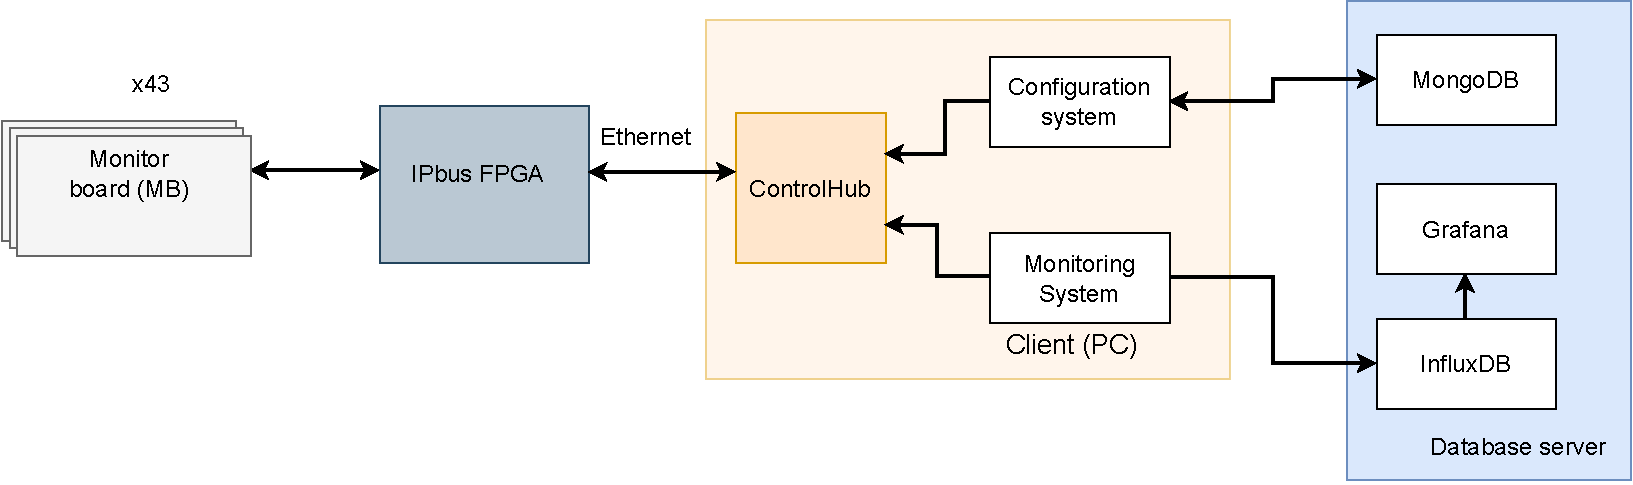
\includegraphics[width=15cm]{images/PCS overview.pdf}
    \caption{Overview of the PCS, emphasising the client software.}
    \label{fig: software_overview}
\end{figure}
\FloatBarrier



The microcontroller on the \gls{mb} already directly monitors the strings, and turns them off if the threshold values is exceeded, but it is still important to display this information to the user, or else it would be next to impossible to troubleshoot and debug the strings.

\autoref{fig: software_overview} shows the client software in detail. The configuration system and monitoring system is made of custom python classes that uses the IPbus API to communicate with the ControlHub, which in turn communicates with the \gls{fpga} over Ethernet cable. The figure also shows the databases the two systems uses to store data, MongoDB stores configuration sets and InfluxDB + Grafana stores monitoring data and displays it to the user. These two systems will be discussed further in \autoref{section: configuration} and \autoref{section: monitoring}.

The client software functions as the "brain" of the \gls{pcs}, the \gls{fpga} and microcontroller on the \gls{mb} is simple by design and more complicated processes is meant to be performed by the software. Processes such as debugging for faulty strings or transmission tests, is created on the software side. Testing and verification of the \gls{pcs} is discussed more in section ??.

The client software uses IPbus software and \gls{api} to communicate with the \gls{fpga}, which requires setting up the address map of the \gls{fpga} with the IPbus software. Address map of the \gls{fpga} is listed in Appendix \ref{appendix: fpga_map}. IPbus stores the address map of the \gls{fpga} within a module address XML file. The individual module address maps is stored in separate XML-files.  the XML-file for one of the com\_modules is shown in \autoref{fig: xml_example}.

\begin{figure}[!htpb]
    \centering
    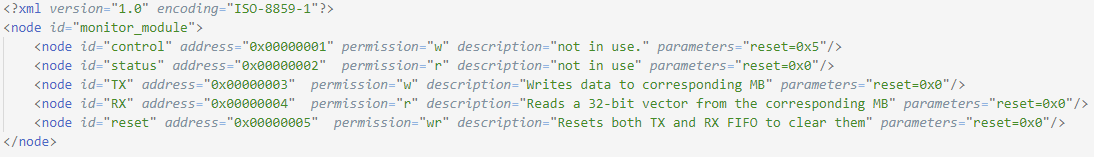
\includegraphics[scale=0.65]{images/com_module_xml.png}
    \caption{XML file of the com\_module used within IPbus software.}
    \label{fig: xml_example}
\end{figure}
\FloatBarrier

The files contain information of each register, such as address, \gls{rnw} access, and a description. IPbus supports additional functions that can be set in the xml-file, but for this project, such functionality is not necessary.

The IPbus \gls{api} consists of ControlHub, a hub that can manage several IPbus clients connected at the same time, and uHAL, which sets up the \gls{api} towards the specified target. The custom Python classes uses uHAL functions for writing and reading registers on the \gls{fpga}; These functions are called \textit{getNode().read()} and \textit{getNode().write()}. When a read or a write function is called, uHAL does not immediately send the data, rather it puts the request in a packet, and when the \textit{dispatch()} function is called, uHAL establishes a connection with the target and sends all requests that was in the packet. This dispatch operation will become important when we start to optimize the transmission speed between software and microcontroller.

Both the monitoring and configuration systems uses \gls{gui}s to interface with the user, but there is additionally a top-level \gls{gui} that unifies both systems. An image of the top level \gls{gui} is shown in \autoref{fig: main_gui}

\begin{figure}[!htpb]
    \centering
    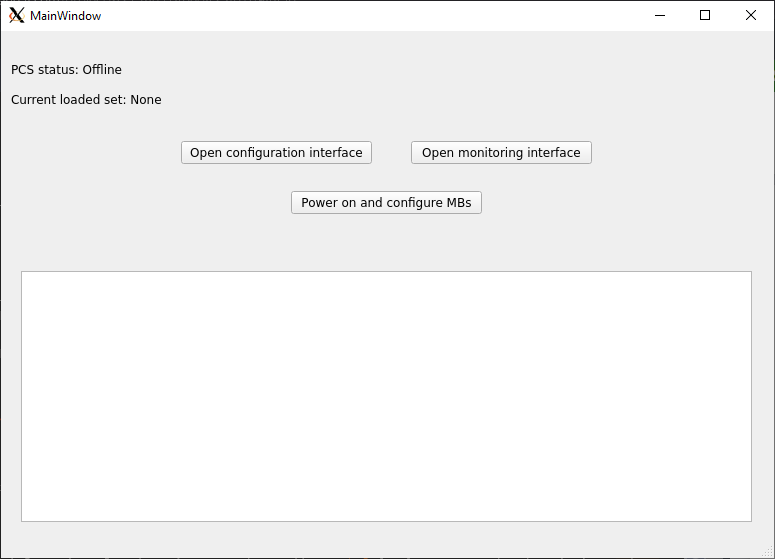
\includegraphics[scale=0.65]{images/main_gui.png}
    \caption{Main hub GUI. Has buttons for opening the monitoring and configuration, starting the configuration, and also contain a logging window.}
    \label{fig: main_gui}
\end{figure}
\FloatBarrier 

The main hub \gls{gui} serves as the top level for the control software, this means the user will boot up the \gls{gui} and can access all functionalities of the control software. This includes setting and creating configuration sets using the configuration \gls{gui}, starting and stopping the monitoring process, opening the Grafana web tool, and finally start the configuration and powering algorithm.

The main hub \gls{gui} has buttons that will open up the configuring and monitoring \gls{gui}s, respectively, and also has a button that will initiate the configuration process. The window also has a logging window to display status and actions performed, to the user

\subsection{FPGA Design}
\label{section: fpga_design}

A communication link between the client software and the \gls{mb} is a necessary part of the \gls{pcs}. A previous paper done for the \gls{pct}-project discussed different design architectures for the \gls{dcs}, which encompasses both chip readout and the \gls{pcs}. A microcontroller based architecture were considered, but it was proven to be too large of a bottleneck in the system. A pure \gls{fpga} architecture was seen as the superior design for the system. The main advantage of using an \gls{fpga}-architecture is the use of IPbus, an Ethernet-based protocol standard. IPbus is designed to read and modify registers within an \gls{fpga} through a communication protocol over ethernet cable, making it suitable for our use.  IPbus was designed to be used in particle physics experiment and is therefore reliable, scalable, and faster than other solutions when sending large amounts of data packets.

An \gls{fpga} must be chosen to be used in the \gls{pcs} and there are certain criteria the \gls{fpga} must meet for this project:

\begin{itemize}
    \item It must have 2*2*43 I/O pins, for communicating with all 43 layers, using \acrshort{lvds}.
    \item \gls{fpga} must be relatively new and still updated, so it will not become obsolete in the coming years.
    \item It must not be too expensive, although this is not a hard requirement, due to only needing one \gls{fpga} for the entire system.
    \item The \gls{fpga} should have an example design for IBbus available, this will cut the development time for the \gls{fpga} design by a large margin.
\end{itemize}

For this project, it was chosen to use the Xilinx Kintex UltraScale KCU105, for meeting all the demands for number of I/O pins and having an example IPbus design available provided by the developers of IPbus.


The \gls{fpga} will be responsible for communicating with the \gls{mb} for each layer. It needs to be able to handle individual read and write for each layer and also have global functions, for broadcasting messages. It will also need to be able to handle errors in case something goes wrong on any of the \gls{mb}s. Several designs were considered for the \gls{fpga}.

The first design is based on having a small module for each layer that communicate with the layer's \gls{mb} and stores data from the microcontroller of its respective layer. The \gls{mb} register data is stored on the module and could be easily read by the client. a TX and RX register in each module is used to transmit data to its respective layer. This design is both simple and modular. Only one small module with relatively little logic needs to be designed and it will be scalable for many layers. A global module would be required to handle broadcast commands for all modules in this design. Note that we are storing all the microcontroller data on the \gls{fpga}, which could be seen as redundant, and more copies of the same data leads to higher chance for errors.

The final design takes the first design and ditches the registers containing the information from the \gls{mb}s, only keeping the two registers for transmitting and receiving data, TX and RX. Each module would therefore only be responsible for sending and receiving data through the TX and RX registers, no direct information of the \gls{mb} is held in the \gls{fpga}. This means that less data is copied, reducing the chance for erroneous data to be stored. The modules would also need a status register for keeping track of eventual errors from the \gls{mb}. The implementation of this design was done by Martin Eggen and Jakob Hauser. The address map for the com\_module and global module is given in Appendix \ref{appendix: fpga_map}. 

These address maps is set in the IPbus module files. Each module on the \gls{fpga} contains a corresponding xml file, in which the address map for the module is set. A figure of their implementation is shown in \autoref{fig: fpga_block}.


\begin{figure}[!htpb]
    \centering
    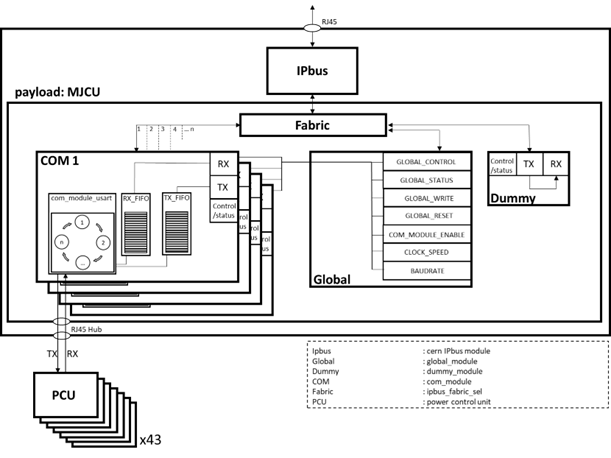
\includegraphics[width=13cm, scale=1]{images/BlockDiagramFPGA.png}
    \caption{Block diagram of the FPGA design. Note that "PCU" is meant to be the MB in the diagram.}
    \label{fig: fpga_block}
\end{figure}
\FloatBarrier

This design has a "com\_module" for each layer that handles write and read transactions to and from the microcontroller using a standard USART protocol. These modules also uses a \gls{fifo} to allow for many data packets to be sent at once, without needing to wait for the module to finish the transmission. The global module has several functions for not only broadcasting, but also can configure universal settings in the \gls{fpga}, such as "global reset" function or setting the baud rate for the \gls{usart}. The global module also contains two registers for enabling and disabling the com\_modules, which will be relevant when we are creating the powering algorithm for the configuration process in \autoref{section: configuration}.

Interfacing with the \gls{fpga} design requires us to know the operations performed by the \gls{fpga} when reading or writing to the microcontroller. When a data packet is sent to the TX register of a com\_module, the \gls{fpga} will send it down to the microcontroller and information from the transaction is always sent to the respective RX register. \autoref{fig: handshake_vals} shows the data flow during a read and a write between the \gls{fpga} and microcontroller.

\begin{figure}[!htpb]
    \centering
    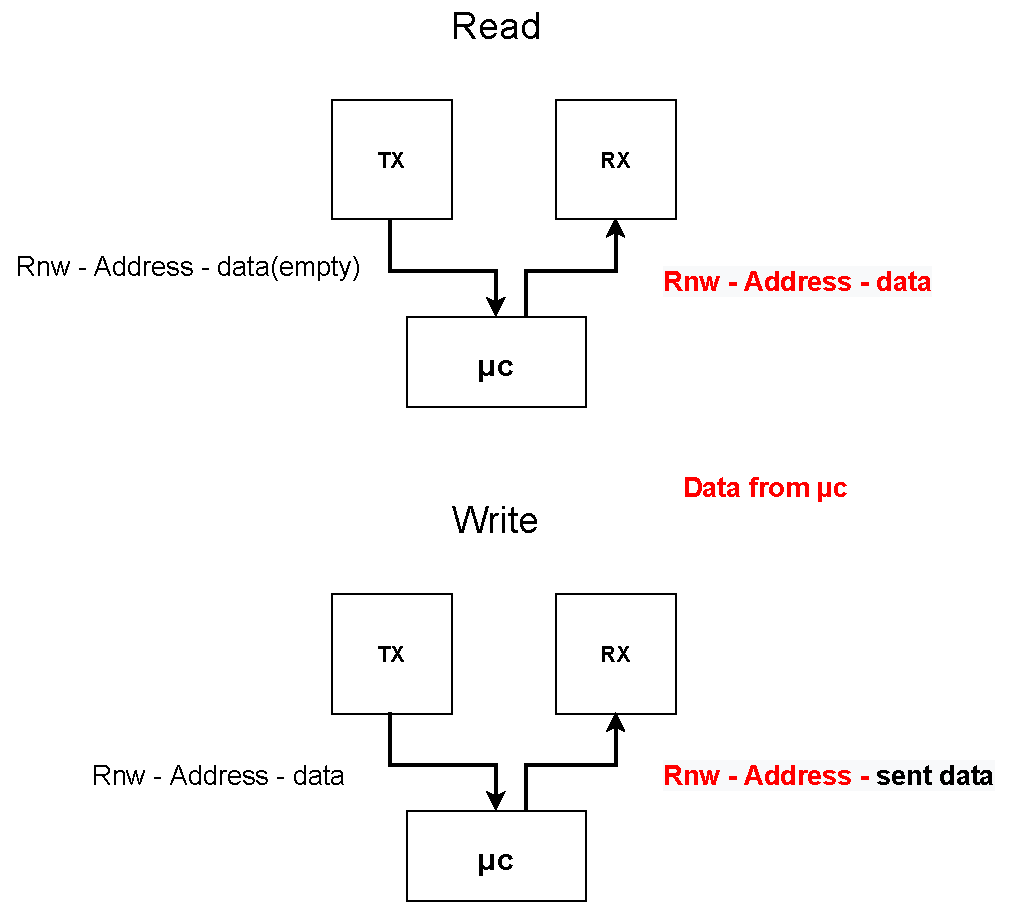
\includegraphics[width=10cm, scale=1]{images/handshake procedure.pdf}
    \caption{Block diagram data flow between FPGA and microcontroller showing handshake values in red.}
    \label{fig: handshake_vals}
\end{figure}
\FloatBarrier

When performing a read, the read data is sent to the RX register along with data of which address was written to, and RnW bit. When performing a write, handshake values from the microcontroller is inserted into the RX register, along with the data sent from TX register. Important to note here that the data value from the write operation originates from the \gls{fpga}, not the microcontroller. These bits will virtually always match up with the sent data packet, and therefore is not interesting to look at when we are debugging for erroneous bits.


\notinmain{husk å source Birger her}
All data written to the TX register of a com\_module is sent down to the microcontroller through 2 \gls{lvds} pins, using \acrshort{usart}. The communication between is described in the timing diagrams of \autoref{fig: master_init} to \autoref{fig: slave_read}

\begin{figure}[!htpb]
    \centering
    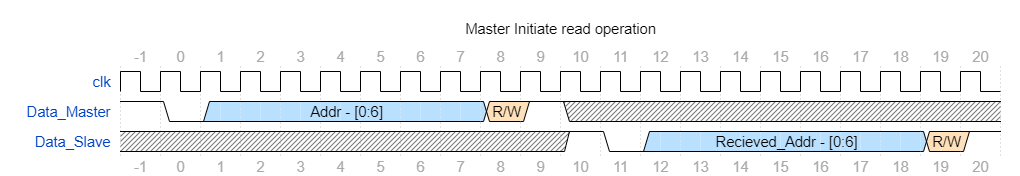
\includegraphics[width=18cm, scale=1]{images/MasterInitRead.png}
    \caption{Timing diagram of Master initializing communication with slave using USART.}
    \label{fig: master_init}
\end{figure}
\FloatBarrier

\begin{figure}[!htpb]
    \centering
    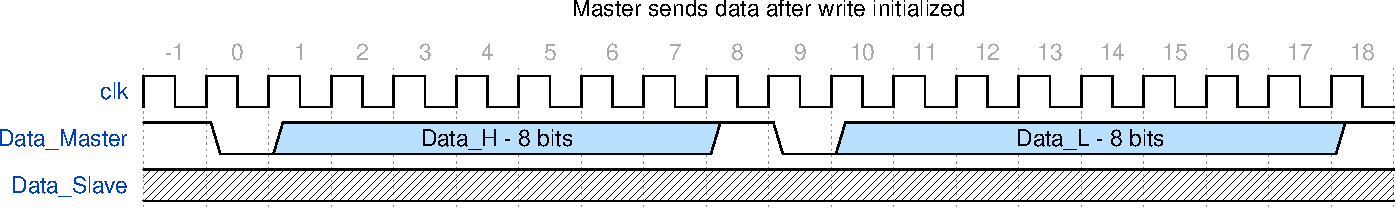
\includegraphics[width=18cm, scale=1]{images/MasterSendData-eps-converted-to.pdf}
    \caption{Timing diagram of Master sending 16 bit data through two packets.}
    \label{fig: master_send}
\end{figure}
\FloatBarrier

\begin{figure}[!htpb]
    \centering
    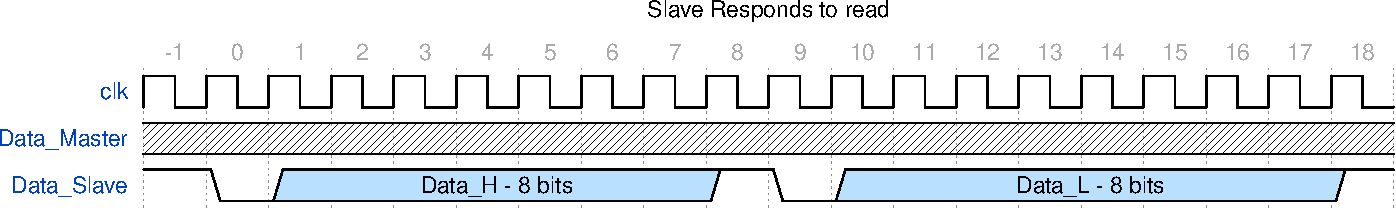
\includegraphics[width=18cm, scale=1]{images/SlaveRespondRead-eps-converted-to.pdf}
    \caption{Timing diagram of Slave sending data after read request.}
    \label{fig: slave_read}
\end{figure}
\FloatBarrier

The master initiates an operation with a start bit and subsequently sends the address value and the RnW bit. The slave performs a handshake by sending the received address back to the \gls{fpga}. The data is always sent with two packets of 8 bits, starting with the high bits and then the low bits. This is done due to the limitations of the microcontroller only having 8 bits per register. \notinmain{legg til bilde av oscilloskop usart kommunikasjon her}.


\notinmain{skriv om data header og hvordan den blir lest, eventuelt skriv om busy signal?}

\subsection{Monitoring Board}
\label{ssec: microcontroller}
The \acrlong{mb} is the board responsible for distributing current to the strings, as well as directly monitoring their current usage and temperature. The board and microcontroller software was developed by Birger Olsen at the same time as this thesis was written. We will not go into detail of the board itself, rather we will focus on the microcontroller software, which the client software will communicate with through the \gls{fpga} translation layer. The board uses an INA3221 chip to deliver DVDD, AVDD, and PWELL current to the strings, and it measures temperature of the strings from a PT100 element.

\notinmain{source birger for bildet}
\begin{figure}[!htpb]
    \centering
    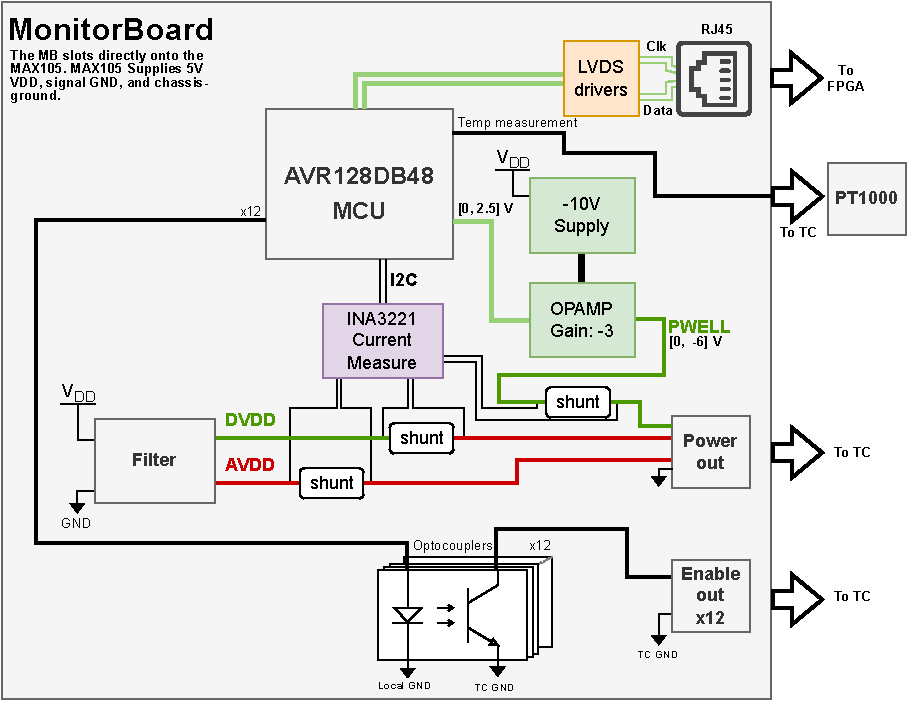
\includegraphics[width=10cm, scale=1]{images/MonitorBoardBlockSchematic.pdf}
    \caption{Simplified block schematic of the \acrfull{mb}}
    \label{fig: mb_schematic}
\end{figure}
\FloatBarrier

The system on the \gls{mb} is controlled by an AVR128DB48 microcontroller, which features a \gls{dac}, an \gls{adc}, I$^2$C and \gls{usart} modules. The AVR128DB also features a  system clock with default speed 4 MHz, but can go up to 24 MHz if needed. As mentioned in \autoref{section: fpga_design}, \acrshort{usart} will be used for communication between \gls{fpga} and microcontroller.

The register map for the microcontroller is given in Appendix \ref{appendix: register_map}. Each register is 8 bit, but the data from the PT100 and INA3221 chip uses 16 bits, therefore each address map uses 2 registers to store the data. The address map consists of threshold level registers, general purpose registers, control registers, and error handling registers.

The data header used to communicate between the \gls{fpga} and microcontroller is 32 bits long, and is made of RnW bit, address, and data to write. The data header is shown in \autoref{fig: tx_header}.

\begin{figure}[!htpb]
    \centering
    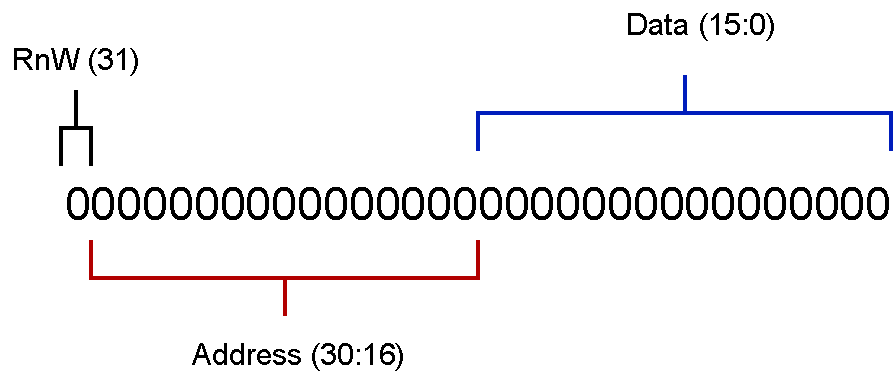
\includegraphics[width=10cm, scale=1]{images/TX packet header.pdf}
    \caption{Data header for communicating with microcontroller}
    \label{fig: tx_header}
\end{figure}
\FloatBarrier

The data bits only have a function during a write operation, during a read, the first 16 bits is not used.

each measurement has two threshold levels, a warning level and an error level. The client software must set these threshold registers when booting up the the strings. The microcontroller will only set an error message if the warning threshold is surpassed by the strings, but it will immediately turn off the strings if the second threshold level is surpassed. When either of the threshold levels is triggered, an error message is sent to the error message register and the error count register is updated.

Checking for errors in the \gls{mb} while monitoring or configuring can be done by reading the error count register in intervals. If an error is detected, then the error messages should be read out by the client software and the error registers can be cleared by writing 0x00 to the error count register.

The microcontroller has 3 control registers, which allows client software to execute custom functions built into the microcontroller, by writing to the registers. This would allow us to perform relatively complex functions, without needing to transmit many data packets through the \gls{pcs}. Functions such as an individual enable scan, which tests the current usage of each individual string, could be performed significantly faster with the use of a custom function on the microcontroller, for example. The control register feature is only in a conceptual state and it has not been fully implemented in the current microcontroller design. CTRL1 register only has a few functions for resetting register values implemented, CTRL2 and CTRL3 is currently unused and has no function.

Functions such as error handling in the control software is not implemented due to the error handling in the 




\notinmain{Skriv om mikrokontroller oppsett, software funksjoner, data header, register map}



\end{document}